\documentclass[10pt,a4paper]{article}
\usepackage[utf8]{inputenc}
\usepackage{amsmath}
\usepackage{amsfonts}
\usepackage{graphicx}
\usepackage{amssymb}
\title{Simulace evoluce}
\author{Prokop Divín}
\begin{document}
\maketitle

\newpage

\tableofcontents

\newpage

\section{Uživatelská část}
\subsection{O programu}

Program přečte předpřipravenou složku kde je nadefinované prostředí a zvířata v něm.
Následně toto prostředí a chování zvířat v něm odsimuluje. Pokud simulace skončí vygeneruje program textový soubor, kde je zaznamenaný průběh simulace (vytištěná ASCI mříž znázorňující stav simulace po každém dnu) a csv soubor, kde je záznam s průměrnými hodnotami zvířat. 
  

\subsection{Pravidla} 
Zvíře musí během dne jíst jídlo nebo ostatní zvířata, pokud je na konci dne jeho hlad větší než snědlo jídla tak zemře. Pokud snědlo dost jídla, to znamená několikrát více než je jeho hlad, tak se rozmnoží. Pokud se rozmnoží vytvoří se nové zvíře, kterému se 
změní jeho vlastnosti(výška, síla smyslů=dohled, pohyblivost) o "mutovací" parametr.

Vlastnosti zvířete ovlivňují jeho hlad, to jak moc záleží na vybrané rovnici hladu.


\subsection{ Ovládání }
Programu je třeba zadat dva parametry. První parametr je cesta k souboru ze vstupními daty. Druhý je název soubory s výstupními daty.
Z názvu souboru pro vstupní data se vytvoří dva soubory. Soubor s příponou ".csv", kde jsou zaznamenané statistiky z jednotlivých dnů simulace a soubor s příponou "\_log.txt", kde je vytisknutý stav simulace po každém dnu.


\subsection{Soubor s parametry}
 Soubor s parametry je textový soubor co udává definici prostředí. Pokud v něm chceme použít komentář, pak
 cokoliv po " \#" až do konce řádku nebude aplikace vnímat.
 
 V souboru můžou být definice tří věcí a to hlavičky, jídla, a zvířete.
 Více definicí jídla znamená více druhů jídla, a u zvířat obdobně.
 Pokud je více definic hlavičky pak platí ta poslední.
 
 
\subsubsection{definice hlavičky}
Toto je příklad zapsání definice hlavičky v souboru. Kde každému parametru patří komentář vysvětlující význam.


\begin{verbatim}
*head  # označuje začátek definice hlavičky
days 50  # počet dnů simulace, totéž jako počet generací 

map_hight 20  # výška mapy 
map_width 25  # šířka mapy 
nutritions_divider 2 #- udává kolik zvířeti zbude z jídla po odečtení jeho                          
                     #  hladu (živiny co zbyly zvířeti se tímto číslem vydělí)
calculator 2 3 4 5 # 2- číslo funkce, která bude počítat hlad 
                   # 3- číslo které určuje jednotky parametru "size" u zvířete 
                   # 4- číslo které určuje jednotky parametru "sense" u zvířete 
                   # 5- číslo které určuje jednotky parametru "dexterity" zvířete 
---------  # ukončuje definici hlavičky

\end{verbatim}

\textbf{calculator x}

Můžeme si vybrat ze čtyř funkcí, kde size, dexterity, sense jsou vlastnosti zvířete, kterému funkce počítá hlad. 


-funkce 0 je inspirovaná vzorcem pro kinetickou energii. 

 $$hlad =(\frac{size}{size_r})^3*(\frac{dexterity}{dexterity_r})^2 +\frac{sense}{sense_r}$$

-funkce 1 nezvýhodňuje žádný z parametrů.

 $$ hlad=\frac{size}{size_r}+ \frac{dexterity}{dexterity_r}+\frac{size}{size_r}$$
 
-funkce 2 zdražuje cenu za sílu smyslů, jinak je jako funkce 0.

 $$hlad =(\frac{size}{size_r})^3*(\frac{dexterity}{dexterity_r})^2 +(\frac{sense}{sense_r})^2$$


Pokud zadáme tedy parametr: \begin{verbatim}calculator 1 2 3 4\end{verbatim} a bude se počítat hlad zvířete s vlastnostmi $size=4,sense=6,dexterity=8$ pak výpočet hladu bude vypadat následovně.

$$hlad=\frac{4}{2}+ \frac{6}{3}+\frac{8}{4}=6$$ 

\subsubsection{definice jídla }
Toto je příklad zapsání definice jídla v souboru. Kde každému parametru patří komentář vysvětlující význam.

\begin{verbatim}

*plant    #musí být první, označuje začátek definice

name p1   # jméno pod jakým uvidíme zvíře v simulaci, musí mít právě dva znaky
		  # kvůli tisku mapy
size 1.01  # pokud zvířete chce rostlinu sníst musí mít větší výšku.

count 25   # počáteční počet rostlin
nourishment 3  # je kolik živin poskytne jeden kus teto rostliny
changer 2 0.85 25 10  # 2..každé dva dny se změní maximální počet jídla,
				               #  do kterého se doplňuje jeho počet na konci dne 
					# 0.85 ...krát se sníží 
					# 25 je maximální počet, kterého může dosáhnout
					# 10 ...je miniální počet kterého může dosáhnout
					# při překročení jedné ze dvou  hranic se jeho počet už 
					# nemění

----- # musí končit  řádkou s alespoň jedním "-"
\end{verbatim}

\subsubsection{definice zvířete}

\begin{verbatim}

*species  # musí být první, označuje začátek definice

name a1 # jméno pod jakým uvidíme zvíře v simulaci, musí mít právě dva znaky
        # kvůli tisku mapy

size 3.5   # výška zvířete
sense 4.2    # jak velký má přehled o okolí. Měří se stejně jako dexterity 
dexterity 5   # a je o kolik polí se pohne za den
reproduction 1.2   # kolikrát víc živin potřebuje aby se rozmnožil (než je jeho hlad)
mutation 0.1   # a je náhodný prvek,číslo od 0-1.
            # Určuje jak moc se budou měnit statistiky při rozmnožení
            # k dané vlastnosti zvířete se přičte  nebo odečte jeho násobek 
food 1.2 2 # 1.2 kolikrát se násobí živiny ze zvířat, když ho sní
			   #  je kolikrát se násobí živiny z rostlin
count 10	   # počet jedinců tohoto druhu  na začátku simulace 
 
stop_eat 1.5  # maximalní počet jídla, které může zvíře sníst se vypočítá takto:
               #  hunger*reproduction*stop_eat....hunger*reproduction*1.5
               
------------  # musí končit řádkou s alespoň jedním "-"

\end{verbatim}


\subsection{Soubor s průběžnými daty}
Je csv soubor, kde je pro každý den záznam. Jeden záznam je jeden řádek.
Pro každou rostlinu tady najdem počet jedinců na začátku dne. Pro každý druh zvířete tady najdem, počet jedinců na konci dne, průměrnou hodnotu parametrů 
"Size", "Sense", "Dexterity".

Zde je příklad: 

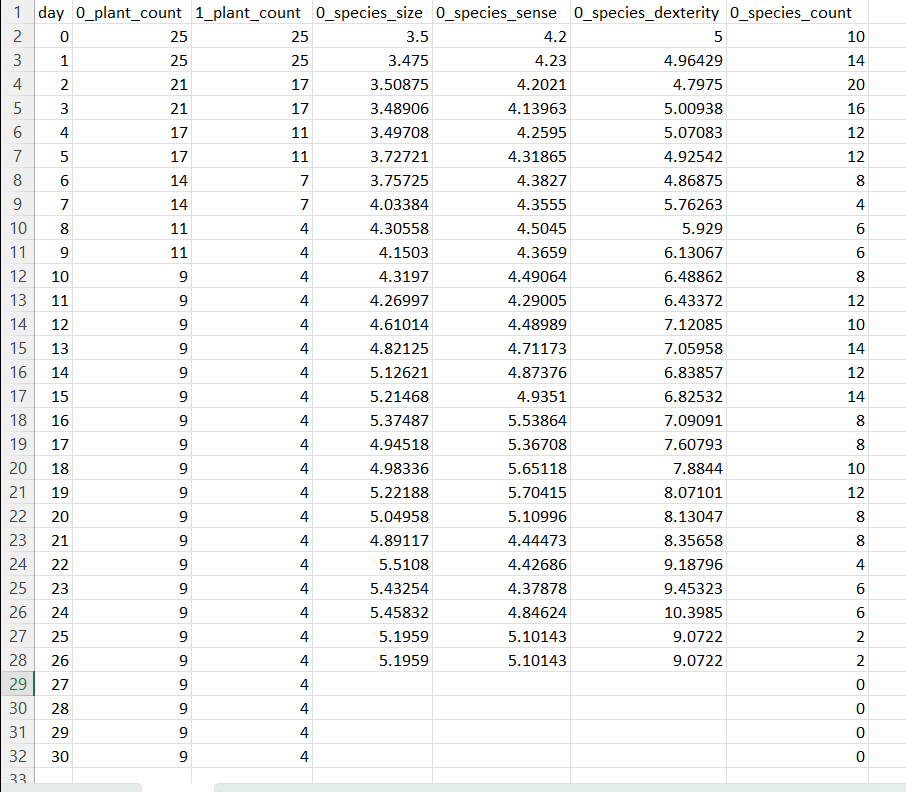
\includegraphics[scale=0.75]{vysledky}


\subsection{Testy}
Všechny testy jsou ve složce tests. V programu hraje velkou roli náhoda. Náhodně se rozhoduje umístění nových zvířat, jídla a změna parametrů při rozmnožování. Proto se Generátor náhodných čísel inicializuje vždy číslem 42.

\subsubsection{Neplatné vstupy}

Tyto testy jsou ve složce errorinputs, mají za úkol otestovat, že program na špatný vstup nespadne a vhodně odpoví.
Po každém z těchto testů by program měl skončit s chybovou hláškou. Testy testují, špatné nastavení parametru případně chybějící nezbytné parametry.

\subsubsection{Platné vstupy}

Na všechny tyto vstupy má program po nějaké době skončit a vytvořit textový soubor se zaznamenaným průběhem simulace a csv soubor s výsledky. Při větších rozměrech mapy doporučuji otevírat textový soubor v editoru který automaticky nezalamuje příliš dlouhé řádky. 

Tyto testy také testují funkčnost komentářů a dalších věcí které by neměli mít na doběhnutí programu vliv. Jako je například rozdílné pořadí sekcí.


Test \textbf{race.txt a race2.txt}

U těchto testů jsou dva druhy zvířat a dva druhy jídla. Jedno můžou jíst jakákoliv zvířata a na druhé musí jedno zvíře alespoň trochu vyrůst, druhý druh je dost velký od začátku. Počet jídla se postupně v průběhu simulace zmenšuje.





Test \textbf{test4.txt, test1.txt, test2.txt, test3.txt}

Tyto testy jsou identické až na druh calculátoru. Můžeme tedy vidět vliv výpočtu hladu na prostředí.

Test \textbf{big.txt}

V tomto testu je mapa 100x100, 3 druhy rostlin a 5 druhů zvířat.
\subsection{Kam dál}

Dále by se dalo zlepšit zpracování výsledků, a to například tak že se podpoří grafickým zpracováním.  K tomu může posloužit csv soubor. Dalším způsobem rozšíření by mohlo být přidání grafického rozhraní nebo nového druhu zvířete s jiným druhem pohybu. 

\section{Závěr}

Při programová mě překvapil rozsah, očekával jsem, že bude program kratší. Přesto, že je program hotov,dalo by se do něj přidat ještě další věci. Jako je například grafické zpracování výsledků nebo přidání zadávání vstupních parametrů rovnou z uživatelského rozhraní. Dále by se dalo více experimentovat s funkcí pro pohyb zvířat a celkově ze způsobem simulování dne. Toto nebylo součástí zadání, je to jen podnět k budoucím pracím, nebo k plánu na dlouhé zimní večery.  

\end{document}